\message{ !name(seminar.tex)}\documentclass{llncs}

%% Verwende A4-Format statt Letter
\usepackage{a4}
%% Deutsche Silbentrennung und Sprache (neue Rechtschreibung)
\usepackage[english]{babel}
%% Verwende Schriftart mit "echten" Umlauten statt Akzenten
\usepackage[T1]{fontenc}
\usepackage{lmodern}
%% Verwende Umlaute direkt
\usepackage[utf8]{inputenc}
%% Hyperlinks für interne Referenzen
\usepackage[]{hyperref}
%% Grafiken einbinden
\usepackage{graphicx}
%% Paket für Unterabbildungen pro Abbildung
%\usepackage{subfig}
%\usepackage[style=alphabetic]{biblatex}
\usepackage{amsmath}
\usepackage{amssymb}
\usepackage{subfigure}

%\usepackage[]{todonotes}
\usepackage{tikz}
%\usepackage{todo}
\newcommand{\todo}[1]{ {\color{red}{\textbf{#1}}}}

\usetikzlibrary{matrix,decorations.pathreplacing}

\DeclareMathOperator{\lsb}{lsb}

%\addbibresource{literature.bib}

% Titel der Arbeit
\title{Extension of Two-Party Computation to Multi-party Computation}
\subtitle{Principles and Applications of Secure Multi-Pary Computation}

% Angaben zum Author
\author{Philipp Müller}
\institute{%
   Fakultät für Informatik, \\
   Technische Universität München \\
%    Munich, Germany\\
   \email{muellerp@in.tum.de}
}

\pagestyle{plain}

%------------------------------------------------------------------------------
\begin{document}

\message{ !name(seminar.tex) !offset(-3) }


\maketitle

%------------------------------------------------------------------------------
\begin{abstract}
We explain how $n$ parties can evaluate a function $f(x_1,\dots,x_n)$ such that each party privately holds one input parameter to the function. The function is evaluated in a manner that ensures that the privacy of each parties input is preserved and only a constant number of rounds is needed.
\end{abstract}

\todo{Secret sharing etwas eingehender beleuchten.}
\todo{Collaborative XOR-Evaluierung (no any number of bits).}
\todo{Explain what it means to \emph{commit} something.}
\todo{One way function exists $\Rightarrow$ pseudorandom generator exists.}
\todo{Parity bit ``defines which gate label to use''!}
\todo{Definieren, was ``secretly and privately computing'' bedeutet.}

%\listoftodos{}

%------------------------------------------------------------------------------
\section{Introduction}
\label{sec:introduction}

Collaborative secure function evaluation has surprisingly many applications in practice. Whenever several participants want to compute some value from their respective inputs and privacy is a concern, we might need a particular scheme to solve some particular problem.

\subsection{Two motivational problems}
\label{sec:motivational-problems}

We will now see two examples of what such problems might look like.

\subsubsection{Secure auctioning}
\label{sec:intro-problem-secure-auctioning}

Imagine the following scenario: Two people ($A$ and $B$) want to buy some good $C$. Of course, the better offer will win, so both $A$ and $B$ are interested in who had the higher bid. However, $A$ and $B$ don't want each other to know the bids, i.e. $A$ wants to keep its bid secret from $B$ and vice versa. Assume $A$ and $B$

We can model this problem as a function

\begin{equation}
  f(a,b)=
  \begin{cases}
    -1, & \text{ if } a>b \\
    0, & \text{ if } a=b \\
    1, & \text{ if } a<b
  \end{cases}.
\end{equation}

Staying within this context, we want to know the function value $f(a,b)$, where $a$ and $b$ denote the bids of $A$ and $B$, respectively, but don't want $a$ and $b$ to become publicly known.

Of course, we might not only be interested in a function $f:\mathbb R ^2\rightarrow \left\{ -1,0,1 \right\}$, but in a function $g: \mathbb R ^n \rightarrow \left\{ 1,2,\dots,n \right\}$ that can be used if not only two, but $n$ people ($A_1,\dots,A_n$) are interested in some good $C$. The output of function $g$ then denotes which person's offer was the best.

\subsubsection{Office assignment problem}
\label{sec:office-assignment-intro-problem}

This problem is taken from \cite{Rogaway:1991:RCS:888502}. Imagine $2n$ people that shall be distributed onto $n$ offices, i.e. one office is shared by two people. Each person $i$ writes a list with values $^iL^j\in [0,1]$ (for $j=1:n$). The value $^iL^j$ denotes how good person $i$ likes person $j$. The higher the value the better.

Of course, they want to be distributed in such a way that their preferences are respected to a certain degree. They agree that for a room assignment $M$ the value
\begin{equation*}
\sum_{\left\{i,j \right\}\in M}\min(^iL^j, ^jL^i)
\end{equation*}
is a good measure for the goodness of the assignment $M$. So, the goal will be to minimize this measure, but -- of course -- no student wants to reveal his preferences (i.e. all the values $^iL^j$ shall stay private to person $i$).

\subsection{Common ingredients of these two problems}
\label{sec:introductory-common-ingredients}

As we saw, in the above two functions, we wanted to compute some value from inputs that were contributed by different parties. Moreover, we -- in particular -- should look out that these inputs shall not become public.

Each participant wants to know the output, but does not want his input to the function to become public. The other way around, no participant shall gather information about the other participant's inputs.

At this point it is worth noting that even the function value itself \emph{might} reveal some information about the inputs. For example, consider $mult(a,b)=a\cdot b$: If $mult(a,b)=0$, one can conclude that one of the arguments must have been zero. Such conclusions -- obviously -- can not be avoided since we are interested in the actual output of the function, that in this case might reveal information about the inputs. However, we want to keep ``as much as possible'' secret. To define what this means precisely is some crucial point that will be adressed later.

This kind of problem can be solved using \emph{secure multi-party function evaluation}. Of course one might tailor a specific scheme for each function. However, it might be of greater value to derive one technique that allows for arbitrary functions.

\subsection{What we will construct}
\label{sec:our-goal}

We will construct a framework that enables some participants (also called \emph{players} or \emph{parties}) to collaboratively evaluate a function such that each participant supplies one input to the function. Moreover, we will address the problem that the inputs shall not be revealed to the community.

Such a protocol for secure function evaluation usually evolves in \emph{rounds}. In each round, the participants can communicate with each other. Between the rounds, they can carry out local computations.

One might be tempted to guess that ``more complicated'' functions take more time to be collaboratively evaluated. However, as we will see, this is not the case. The protocol we describe takes a constant number of rounds (independent of the function) and keeps the amount of communication between the single participants polynomially bounded.

\section{Formal definitions for Secure Computation}
\label{sec:formal-definition}

We said that we want to compute functions in a way such that the inputs stay private to the respective players. We call that $secure$. While this colloquial explanation is quite intuitive, we will briefly examine what it means formally. The following definitions are along \cite{Rogaway:1991:RCS:888502} and \cite{Beaver1990}.

\subsection{Prerequisites}
\label{sec:prerequisites}

\paragraph{A word on the security parameter.}

A central value when considering cryptographic schemes or protocols is the so called \emph{security parameter}, often denoted by $k$. In short, this is some constant that is fixed before setting up some cryptographic algorithm or protocol\footnote{That is, you pick some security parameter, and afterwards the cryptosystem is set up according to this parameter.}. The run times of encryption/decryption or the runtimes needed by some adversary are then typically measured as a function in $k$.

Informally stated, typically the following is the case: As soon as $k$ is greater than some particular value, the system constructed (according to this parameter) is considered secure (see \cite{lecture-notes-goldwasser-bellare}).

\begin{definition}[Negligibility]
  A function $\epsilon:\mathbb{N}\rightarrow\mathbb{R}$ is \emph{negligible} if $\epsilon(k)\in k^{-\omega(1)}$.
\end{definition}

To bring the notion of negligibility in a format that is (due to Landau-Notation) possibly more well-known to most computer scientists, we can say, that a function $\epsilon(k)$ is negligible, if for every positive integer $c$ there exists some $k_0$ such that for all $k>k_0$ we have $|\epsilon(k)|<k^{-c}$ (so: $\epsilon$ negligible $\Leftrightarrow \forall c>0.\ \exists k_0.\ \forall k>k_0.\ \epsilon(k)<k^{-c}$, see \cite{bellare-hoang-rogaway-garbling-schemes}). That is, a function $\epsilon(k)$ is negligible if it vanishes faster than any polynomial-inverse.

A typical example for a function that vanishes faster than any polynomial-inverse is $f(k)=2^{-k}$. This is a function that grows inverse-exponential.

As you can see, we already specified $\epsilon$ as a function of $k$ (which stands for the security parameter). This is because negligibility is a tool that is often applied to e.g. the success probability of an adversary's attack.

\paragraph{Alphabets and strings.}

Let us \emph{informally} introduce alphabets and strings, since they are -- at least at the level of definition -- quite intuitive. We call some set $\Sigma$ of letters an \emph{alphabet}. If we take several letters from this alphabet and concatenate them, we obtain a \emph{string} over the alphabet $\Sigma$. If there's no risk of confusion (which is almost always the case) we omit the phrase ``over the alphabet $\Sigma$'' and just call it ``string''. Moreover, we use no special sign for concatenation, but just write one letter after another.

There is exactly one string consisting of no letters at all (the empty string). By $\Sigma^l$ we denote the set of all strings of length exactly $l$. We define the set of \emph{all} strings over some aphabet $\Sigma$ by
\begin{equation*}
\Sigma^*=\Sigma^0\cup\Sigma^1\cup\Sigma^2\cup\Sigma^3\cup\dots=\bigcup_{i=0}^\infty\Sigma^i.
\end{equation*}

For our needs, we will consider $\Sigma=\left\{ 0,1 \right\}$, which is not a real restriction, because everything can be represented using only bytes (without blowing up the representation \emph{too much}).

We call every subset of $\Sigma^*$ a (formal) \emph{language}.

\paragraph{Probability measures over languages.}

In order to understand the next definition, we have to think about the following random experiment: Take $\Sigma^*$ and pick some string randomly from it. The so-called \emph{probability measure} then ``tells us'' for each string how probable it is to pick exactly this string. That is, it maps each string (and -- by extending it -- every set of strings) to some probability between 0 and 1.

\begin{definition}[Ensemble]
  We call a family of probability measures $\{{\cal A}_k\}$ on $\Sigma^*$ an \emph{ensemble}, if only strings of length of at most $q(k)$ have positive probability with respect to ${\cal A}_k$, where $q(k)$ is some polynomial in $k$.
\end{definition}

The notation $\left\{ {\cal A}_k \right\}$ should be understood as the set
\begin{equation*}
\left\{ {\cal A}_k \mid {\cal A}_k \text{ is a probability measure on } \Sigma^*, k\in\left\{ 0,1,2,3,\dots, \right\} \right\}.
\end{equation*}

So, a probability measure in an \emph{ensemble} ``operates'' only a \emph{finite subset} $S$ of $\Sigma^*$ (since it only ``maps'' strings of length of finite length onto nonnegative probabilities), and ``randomly picks'' a string from this finite set $S$ according to its distribution.

\begin{definition}[Indistinguishability]
  For ${\cal A}$ taken from some ensemble and $C$ a boolean circuit (having sifficiently many inputs), $p_{\cal A}^C$ denotes the probability that $C$ outputs 1 on an input randomly drawn according to the distribution given by ${\cal A}$.

  We say that ensembles $\left\{{\cal A}_k\right\}$ and $\left\{{\cal B}_k\right\}$ are \emph{computationally-indistinguishable} if for any polynomial-size circuit family ${\cal C}=\{C_k\}$, the function $\epsilon(k):=|p_{{\cal A}_k}^{C_k}-p_{{\cal B}_k}^{C_k}|$ is negligible.
  
  We call ${\cal A}$ and ${\cal B}$ \emph{statistically indistinguishable} if the function 
  \begin{equation*}
\epsilon(k):=\max_{S_k\subseteq \Sigma^*}|\Pr_{{\cal A}_k}[S_k]-\Pr_{{\cal B}_k}[S_k]|
\end{equation*}
is negligible, where $\Pr_{{\cal A}}[S]$ denotes the probability that we get a string within $S$ if we draw from $\Sigma^*$ randomly according to the distribution ${\cal A}$.
\end{definition}

Essentially, if two ensembles ${\cal A}$ and ${\cal B}$ are \emph{computationally} indistinguishable, then no efficient (i.e. no polynomial-time) algorithm can decide whether a sample given to it came from ${\cal A}$ or ${\cal B}$. In other words, any efficient algorithm's behaviour doesn't change significantly when given samples from ${\cal A}$ or ${\cal B}$, respectively. Note that statistical indistinguishability is a stronger property then computational indistinguishability in the sense that statistical indistinguishability implies computational indistinguishability.

For more information on indistinguishability, please refer to e.g. \cite{goldreich_foundations_of_crypto_2}.

For us, distinguishability is ``just a tool'' that helps us analyzing whether some malicious agent who is attacking our protocol can distinguish the protocols outcome from some sample obtained by some randomized algorithm. We will come to that later in more detail.

\subsection{Model of computation}
\label{sec:model-of-computation}

We assume a synchronous model. In this setting, the participants can either broadcast a message to everybody or use a private channel to one specified receiver. We imagine this as a network of processors whose computation is controlled by a common clock ticking (at time steps $0,1,2,\dots$). We assume local computation to be ``instantaneous'' compared to the clock ticks, i.e. whenever some participant computes something \emph{locally}, we do not consider the exact runtime of this operation, but we just assume that particular computation to take exactly the time between two rounds. Round $i$ starts at tick $i$ and lasts until tick $i+1$.

\paragraph{Communication between participants.}

We assume a read-only common input tape for all participants that contains (among others) the security parameter $k$ (in suitably encoded format). We assign each player a private work tape (read/write), a private read-only input tape and a private write-only output-tape, all of which are initially empty. 

Moreover, we assume that between any two participants $i$ and $j$ there is a private channel $i\rightarrow j$ to securely send messages from $i$ to $j$. This can be seen as a write-only tape for $i$ and a read-only tape for $j$. These private channels are organized in a way such that the receiver can determine who sent the corresponding message.

Last, each player has a broadcast channel (write-only for the sending participant, readable by everybody).

It is convenient to assume that at each time step, there is a well-defined (possibly empty) message on each channel (i.e. in particular on broadast and private channels).

Additionally, each player has access to a fair coin to support nondeterminism.

Player $i$ runs program $P_i$, so that we call the tuple ${\cal P}=(P_1,\dots,P_n)$ a \emph{protocol}. The \emph{history} of player $i$ consists of everything player $i$ had access to (coin tosses, messages sent and received, private and ocmmon input).

\paragraph{Round and communication complexity.}

We stated that a protocol proceedes in rounds, and in each round participants might (or might not) communicate with each other. ``In between two rounds'', the participants have the possibility to do local computations. For collaborative function evaluation, the number of rounds together with the amount of communication is the decisive point. That is, when we consider a protocol's complexity, we have to distinguish between \emph{round complexity} (i.e. the number of rounds needed by the protocol) and \emph{communication complexity} (i.e. the amount or length of messages exchanged by the individual participants). Note that the number of rounds is usually the crucial size we try to keep low.

\subsection{Adversaries}
\label{sec:adversaries-more-detail}

\paragraph{Power of adversaries.}

In particular, we are interested in what happens if not all players are following the protocol. We will have to explain how to proceed if some of the players are corrupted by an adversary (e.g. some malicious agent).

Therefore, we have to define what the participants of our protocol can do (and what they can't), and what a so-called \emph{adversary} might do in order to compromize our privacy or disrupt correctness of our protocol. On the other hand, we -- of course -- need to describe how to tackle such adversaries.

In our case, we assume quite strong adversaries, that can ``infect'' players so that the adversary knows the players whole ``state'' and controls all future actions of the infected players. 

Moreover, we will consider adversaries that can infect players not only at some statically defined point of the protocol, but can act somewhat \emph{dynamically}. The type of adversary we are considering is called a \emph{uniform} adversary. That means, an adversary $A$ is a probabilistic polynomial-time algorithm. An adversary infects or ``corrupts'' players. We consider adversaries that can do so at the beginning of each new round. Note that such an adversary can -- after he infected one player -- decide whether to infect another or not.

However, we apply one restriction: The number of players an adversary can corrupt is bounded by some value. We call this value $t$. An adversary is called $t$-adversary if he corrupts at most $t$ players.

%Therefore we will consider adversaries that can -- after infecting some player -- decide whether they want to infect other players or not. They have the possibility to do so at each beginning of a new round. 

After an adversary has infected a participant, it controls the player fully.

Note that we won't consider many distinct adversaries ``within'' one protocol, but we assume only \emph{one} single adversary attacking or protocol. That is no real restriction, since we can interpret several malicious agents as ``belonging'' to one malicious instance only.

\paragraph{What does it mean to defeat an adversary?}

Imagine a black-box that computes some function privately and securely and that is resistant against attacks from adversaries. We say that a protocol computes a function securely if it -- under attack by the adversary -- imitates this black-box under attack as closely as possible. To formalize this in a mathematical way is a clearly non-trivial issue. We will address this later and see what it means in more detail. For now, we just say that an adversary should not be able to decide whether some information come from a randomized algorithm (a so-called \emph{simulator}), or the information comes from a real protocol that he was trying to compromise.

We assume that the protocol ends as soon as all uncorrupted participants have terminated. Then the adversary terminates, too. At this time the tape of the adversary has some string on its output tape. If we consider the protocol ${\cal P}$, security parameter $k$ and the private inputs $\overrightarrow{x}=(x_1,\dots,x_n)$ as fixed instances, the adversary $A$ defines a probability space $\mathbf{VIEW}_A^k(\overrightarrow{x})$ of adversary outputs. We can interpret the adversary's output as an encoding of its history (that is of coin flips, received and sent messages, etc.).

Moreover, each player has output a certain value. We the output values of the uncompromised players by $\mathbf{OUTPUT}_A^k(\overrightarrow{x})$. When we are interested in a sample from this distribution, we just consider the outputs of non-infected players.

\subsection{Security}
\label{sec:definitions-security}

As mentioned before, we want that ``the adversary doesn't know whether what it sees comes from the protocol, or from some randomized algorithm (a so-called \emph{simulator})''. That is, we want that the adversary's view can be \emph{approximated} by a simulator. One question is, what auxiliary tools this simulator can use to approximate the view. We will consider simulators that have access to a so-called \emph{oracle}:

\begin{definition}[$t$-bounded oracle]
  A $t$-bounded $(\overrightarrow{x},f)$-oracle is an oracle accepting two kinds of queries:
  \begin{description}
  \item[Component query] A component query is an integer $i\in \{1,2,\dots,n\}$. If is only answered if $t$ or fewer component queries were made so far. If this is the case, the oracle distinguishes:
    \begin{itemize}
    \item If there was no output query so far, it is answered by $x_i$.
    \item If there was already a proper output query (see below), namely $\overrightarrow{x}'_T$, the query is answered by $(x_i,f_i(\overrightarrow{x}_{\overline{T}}\cup\overrightarrow{x}'_{T}))$.
    \end{itemize}
\item[Output query] An output query is a ``tagged vector'' $\overrightarrow{x}'_T$ (see below). It is answered by $f_T(\overrightarrow{x}_{\overline{T}}\cup\overrightarrow{x}'_{T})$ if $T$ consists precisely of the component queries made up to now and if there were not output queries so far. Further or improper output queries stay unanswered.
  \end{description}
\end{definition}

The first thing we have to clarify is the meaning of a tagged vector. Consider vectors $\overrightarrow{v}=(v_1,\dots,v_n)$ and $\overrightarrow{w}=(w_1,\dots,w_n)$ and some set $T\subseteq \left\{ 1,2,\dots,n \right\}$. Then, the $T$-tagged vector $\overrightarrow{v}_T$ is defined by $\left\{ (i,v_i) \mid i\in T \right\}$. That is, a tagged vector is a set of pairs each containing an index and an actual element. Please note that if each index is present exactly once in some tagged vector, it can easily be seen as a ``usual'' vector (simply by writing the elements at the specific positions). This means, that (with $\overline{T}=\left\{ 1,2,\dots,n \right\}\setminus T$) we can interpret $\overrightarrow{v}_T\cup \overrightarrow w_{\overline{T}}$.

Note that there might be component queries after an output query, as long as the number of component queries does not excede $t$.

As you can see, an oracle is parametrized with $t$, $\overrightarrow{x}$ and $f$, i.e. it can be  specifically designed for the function $f$ we are interested in and the corresponding input values (encoded in $\overrightarrow{x}$). Moreover, it essentially allows up to $t$ component queries. Remember that we didn't allow an adversary infecting as many players as he'd like to, but we limited the number of infected players to $t$.

We consider simulators $S$ having access to a $t$-bounded $(\overrightarrow{x},f)$-oracle. We denote the output of simulator $S$ by $\textsc{Output } S^{O_t(\overrightarrow{x},f)}(1^k)$. Note that this -- again -- forms a probability space. That is, fixing $k$, $f$ and $\overrightarrow{x}$, and ``generating'' some random result by applying $S$ with these parameters, we get a value according to some random distribution.

By $\textsc{Queries } S^{O_t(\overrightarrow{x},f)}(1^k)$ we denote a pair containing the following two things:

\begin{itemize}
\item The indices $i$ for which there was \emph{never} a component query, i.e. it contains the components that were never queried by $S$.
\item The (single) output query that was made by $S$.
\end{itemize}

Since $S$ is a simulator (a randomized algorithm), it might randomly and dynamically decide which components to query and \emph{when} to do an output query. Thus, $\textsc{Queries } S^{O_t(\overrightarrow{x},f)}(1^k)$ forms a probability space, as well. 

An element from this probability space is written $(G,\overrightarrow{x}'_{T})$, where $G$ denotes the indices that were \emph{never} queried by $S$ and the $\overrightarrow{x}'_{T}$ is the output query (remember: there can only be \emph{one} output query). As you can see, $G$ may be a proper subset of $\overline{T}$.

You see, we defined several probability spaces for adversaries as well as for simulators. We shall now see, why we did so and what we consider ``secure'':

\begin{definition}[Privacy, Correctness]
  Let $f:(\Sigma^l)^n\rightarrow(\Sigma^l)^n$. A protocol ${\cal P}$ $t$-securely computes $f$ if for all $t$-adversaries $A$ there exists a simulator $S$ (probably using a $t$-bounded oracle) such that the following hold:
  \begin{description}
  \item[Privacy] For all $\overrightarrow{x}\in(\Sigma^l)^n$, the $k$-parametrized ensemble $\mathbf{VIEW}_A^k(\overrightarrow{x})$ and the ensemble $\textsc{Output } S^{O_t(\overrightarrow{x},f)}(1^k)$ are computationally indistinguishable.
  \item[Correctness] For all $\overrightarrow{x}\in(\Sigma^l)^n$, the $k$-parametrized ensembles $\mathbf{OUTPUT}_A^k(\overrightarrow{x})$ and $[(G,\overrightarrow{x}'_T) \leftarrow \textsc{Queries } S^{O_t(\overrightarrow{x},f)}(1^k)\mid f_G(\overrightarrow{x}_{\overline{T}}\cup\overrightarrow{x}'_T)]$ are statistically indistinguishable.
  \end{description}
\end{definition}

We see that we require (for privacy) that -- intuitively -- the outcome of an adversaries computation can be \emph{simulated} by some random algorithm (that has access to some oracle). The thought behind is the following: ``If the adversaries computation could have been done by a simulator (not even knowing the protocol), then the adversaries attack couldn't be that useful.''

The above definitions state that for any adversary $A$ there is some simulator $S$ that fulfils the privacy and correctness criteria for this particular adversary. I.e. it is enough if there is (at least) one simulator for each adversary, and different simulators might be used for different adversaries. That is, from the definition, one might taylor the simulator to the specific given adversary.

However, as \cite{Rogaway:1991:RCS:888502} proved, our construction leads to something stronger, namely \emph{one} single simulator that works for \emph{all} adversaries (or at least for all the ones that we allowed). %This is achieved using the following construction: The simulator itself uses adversary $A$ and lets it act in the simulators ``virtual world'' that simply emulates the real network. That is, $A$ sees an indistinguishable view of te real world. The simulator let's $A$ work on its own. After the internal world terminates, the simulator returns what its internal adversary ouputted in the virtual execution.\todo{Maybe we need some stuff from the original paper here.}

\subsection{What can we use as a basis}
\label{sec:building-blocks-for-the-protocol}

As we will see, we won't construct the protocol ``from scratch'', but we will use other, already established techniques to solve the problem. These are nowadays well-known concepts, that we present here briefly.

\paragraph{Secret sharing.}

If we want to compute a function collaboratively, it is, of course, advantageous if we are able to distribute information across players. As said before, each player will hold some private input (which we call -- for now -- her \emph{secret}).

Therefore, it is useful that a single player can ``split up'' her secret into small pieces that can be distributed among all players. 

The clou is, that this secret is split up in a way such that -- essentially -- none of the players can reconstruct the secret on his own (i.e. from his single part only), and the secret can only be reconstructed if a certain amount of players are joining and revealing their parts of the secret. 


If you can't imagine how this could even work, you might have a look into section \ref{sec:appendix-basic-idea-secret-sharing} in the appendix --- or even better into e.g. \cite{shamir_secret_sharing}.

We call the player holding the secret the \emph{dealer} and call the distributed parts \emph{shares}.

\paragraph{Verifiable secret sharing.}

We call secret sharing \emph{verifiable}, if the dealer is not able to distribute incorrect shares to the other players and even some dishonest players are tolerated. More precisely, it is ensured that even if the dealer is malicious, the other players can later reconstruct some well-defined secret.

We consider a dealer $D$ holding a secret bit $b$ that is engaged in a verifiable secret sharing scheme tolerating up to $t$ faults. After the scheme, each player $i$ holds his own private share $b_i$ of $b$. Then, we require three properties:

\begin{enumerate}
\item With high probability (i.e. greater than $1-2^{-k}$, where $k$ being the security parameter), there exists a unique value $b'$ such that if the good players broadcast their private shares, each good player will locally compute $b'$ from the broadcasted values, regardless of the values broadcasted by malicious players.
\item If the dealer is good, then the computed value $b'$ will be the correct value $b$.
\item If the dealer $D$ is good, then the view of any adversary not corrupting $D$ is independent of $b$. That is, there is some simulator \emph{independent} of $b$ that can simulate the adversaries view.
\end{enumerate}

If player $D$ splits up his secret $b$ and distributes it, we say that $D$ \emph{commits} to $b$. After $D$ commited to $b$, $b$ is said to be \emph{commited} or a \emph{shared} secret. One important aspect of commiting is the following: If a dealer commits to a certain value, then this value is not automatically known publicly (it is just shared). But the dealer can not change his mind afterwards, that is, once he commits to a value, he is ``bound'' to that value. For more information on this topic, we refer to section \ref{sec:dealer-bound-to-commited-value} or \cite{lecture-notes-goldwasser-bellare}.

Even if we defined verifiable secret sharing for single bits, we can easily extend it to strings, if we simply share each bit of the corresponding string.

For more information on verifiable secret sharing, please refer to e.g. \cite{verifiable-secret-sharing-chor-ben-gold-sha-mic}.

It has been shown that -- in our model of computation -- verifiable secret sharing can be implemented in a constant number of rounds in the presence of a $t$-adversary for $t<n/2$. If you are interested in the proofs of these statements, please consult \cite{rabin-ben-or-verifiable-secret-sharing-number-rounds,beaver-verifiable-secret-sharing}. 

\paragraph{Computing on shared bits.}

As we will later see, circuits are a basic construct when we evaluate a function. It has been proven, that a boolean circuit (representing some function) with bounded fan-in and depth $d$ can be evaulated securely and secretly in $O(d)$ rounds involving an amount of communication that is polynomial in $k$ and in the size of the circuit. That is, we can assume that the inputs to the circuit and the result of the evaluation of the circuit are shared bits (and thus not publicly known). If you are interested in the proofs of these statements, please consult \cite{rabin-ben-or-verifiable-secret-sharing-number-rounds,beaver-verifiable-secret-sharing,how-to-play-any-mental-game-goldreich-micali-wigderson}.

The problem with these protocols is that they do not necessarily work in a constant number of rounds. Our protocol will overcome this weakness, but relies -- in some intermediate steps -- on those protocols.

\paragraph{Collaborative coin flipping.}

Flipping coins collaboratively can be seen as a special case of the previous problem, added some randomness. It allows a group of players to obtain shared random bits (that then are known to \emph{nobody}!). They can be constructed if each player commits a random bit. Then, the participants could -- if they (or at least some specified subset of them) revealed their shares -- recompute each single bit commited by all the participant. For a brief introduction on how this works, you might have a look at section \ref{sec:appendix-coin-flipping}.

\paragraph{Proving assertions to the community.}

In our protocol, players will need to assert that some of their local computations were done right. Proving correctness can be done fast, even if the corresponding computation might have involved deep circuits.

Informally, if we have a function $f:\Sigma^a \rightarrow\Sigma^b$ represented by a circuit $C$, and shared input bits $\sigma_1,\dots,\sigma_a$, then a player can commit $f(\sigma_1,\dots,\sigma_a)$ to prove that he computed $f$ on the given bits correctly. This proof information-theoretically reveals nothing and requires $O(1)$ rounds and a polynomial amount of communication (in $|C|$ and $k$).

When the player proves correctness of his computation, she commits (additionally to the function value) some certificate containing the internal values of the wires. 

%\todo{Aufzeigen, wo das im Protocoll benötigt wird.}

\paragraph{Pseudorandom generators.}

As we will see later, we will use so-called pseudorandom generators in the protocol. A pseudorandom generator is a \emph{deterministic} algorithm running in polynomial time that takes a ``seed'' (some truly random string) as input and composes a longer, pseudorandom string from it (``stretching''). Thereby it shall hold the following: The output of a pseudorandom generator can not be distinguished from a truly random source (in the formal definition, we use negligibility to state this).

Note that a pseudorandom generator has the property, that we can not deduce its input from its output. Functions that have this property are also called \emph{one-way functions}.

Even if it is not known for sure that such generators exist, it has already been proven that they at least exist under very convenient complexity-theoretic assumptions. For more information on this topic consult \cite{pseudorandom-generators-blum,pseudorandom-generators-yao}

\section{The protocol on a very high level}
\label{sec:high-level-description}

In order to understand how the protocol works, we now consider the involved strategy on a very high level. Later, we will give a more formal version (i.e. essentially an algorithm) for the protocoll.

\subsection{General idea}
\label{sec:general-idea}

First of all, we are -- as alluded before -- assuming the function to be on hand in a suitable and unified format, namely in shape of a circuit. That is, we represent a function as a collection of gates and wires. The input wires to the circuit will correspond to the (private) inputs $x_1,\dots,x_n$, while the output wires determine the result $f(x_1,\dots,x_n)$ we want to compute. Note that not each $x_i$ is represented by one wire only, since it might well be the case that one single $x_i$ consists of several bits. That means, that each input bit is assigned to one wire.

It is worth noting that we can without loss of generality assume the circuit to consist only of gates having at most 2 input wires. We can reduce any circuit having gates with more than two input wires to such a circuit. This will increase the size of the circuit, but only by a polynomial factor (in the size of the original circuit). For a short explanation, please refer to section \ref{sec:size-two-fan-circuits}. This will simplify our construction. Moreover, we assume that the gates used in that circuit have a special format: Either they have only one output wire, or they have two output wires, but then only one input wire (we will later discuss why this is necessary). Last, we will assume no ``circles'' in our circuit\footnote{That makes sense when we are representing functions -- in the mathematical sense -- by a circuit.}.

At the beginning, everybody knows the circuit, since the function we want to compute is known to all participants.

The first thing we are going to do is constructing a so-called \emph{garbled circuit}. This is a circuit that resembles a computation which is related to the original function $f$ in such a way that one can -- using certain substitutions -- compute the outcome of $f$ without actually knowing the input (and intermediate) values to $f$. To be a bit more concrete, the garbled circuit will not receive the original inputs, but will receive inputs whose \emph{meanings} (or \emph{semantics}) are (mostly) unknown to the computing parties. That is, a participant can actually compute the correct output of the circuit, even though she does not learn the intermediate values. While this might sound strange to the reader, it is really just the idea at a very high level. We will shortly come to the details of this construction.

As we will see, we can use a trick for each gate that enables us to compute the output of the gate (whose semantics will also be unknown). In this way, we can propagate the computation up to the final gate. This will be the only gate whose outputs can be easily associated with their semantics.

In this way, we will be able to finally compute the final gate's outputs and semantics (and hence the function value), while keeping the input and intermediate values secret from anybody else.

Let us briefly summarize the idea as follows: We will construct a scheme that \emph{hides} the actual bits within the circuits. The participants will still use some intermediate signals during the computation, but they will \emph{not know} if a particular intermediate signal represents a bit 1 or a bit 0.

Let us for now consider a concrete example of how we can construct a garbled circuit from an original circuit. Later, we will define the procedure more formally.

\subsection{Concretizing the idea -- an example}
\label{sec:concrete-idea}

\subsubsection{Our example function and its associated circuit.}
\label{sec:our-example-function-and-its-circuit}

To illustrate the transformation of a circuit into a suitable garbled circuit, we present an example which is taken from \cite{Rogaway:1991:RCS:888502}. Consider the function 
\begin{equation*}
  f :
  \begin{cases}
    \left\{ 0,1 \right\}^3 \rightarrow \left\{ 0,1 \right\} \\
    (x,y,z) \mapsto (x \wedge y) \vee z
  \end{cases}
\end{equation*}
and imagine we have three participants (let's call them $X$, $Y$ and $Z$ for the corresponding inputs) that want to evaluate $f$ for their respective inputs.

\begin{figure}[t]
  \centering
  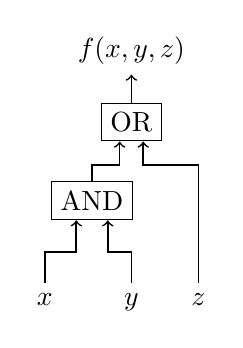
\begin{tikzpicture}
    \node(AND) at (0,1) [rectangle,draw=black] {AND};
    \node (OR) at (.5,2) [rectangle,draw=black] {OR};
    \draw[<-,semithick] (-.2,.75) |- +(-.4,-.4) -- +(-.4,-.8) node[below] {$x$};
    \draw[<-,semithick] (.2,.75) |- +(+.3,-.4) -- +(+.3,-.8) node[below] {$y$};
    \draw[<-,semithick] (0.35,1.75) -- +(0,-.3) -| (AND);
    \draw[<-,semithick] (0.65,1.75) -- +(0,-.3) -| +(.7,-1.8) node[below] {$z$};
    \draw[->,semithick] (OR) -- +(0,0.6) node[above] {$f(x,y,z)$};
  \end{tikzpicture}
  \caption{Circuit computing $f(x,y,z)=(x\wedge y)\vee z$. Note that this (simple) circuit satisfies the requirements we proposed: No circuits, only gates having two inputs and exactly one output.}
  \label{fig:simple-circuit}
\end{figure}

The function $f$ can -- and will -- be represented straightforward by the ciruit $C$ shown in Figure \ref{fig:simple-circuit}. This circuit simply consists of two gates (and some wires connecting these gates properly), one of which is computing the AND of $x$ and $y$, the other one taking the OR of $z$ and the result given by the AND-gate. While this circuit is really simple, we might as well deal with more complicated circuits representing more sophisticated functions, but for demonstration this one is sufficient.

Remember now that we want to compute $f(x,y,z)$ in a way such that no participant can infer more information about the output as the result $f(x,y,z)$ itself implicitly reveals. Since we want \emph{no} participant to gather information about the inputs of the other two players, it is not a good idea to leave the whole computation to one participant alone. Thus, we will compute the function \emph{collaboratively} and thereby take care that no participant has to reveal his input to some other participant.

However, if we operate \emph{directly} on the given circuit, our participants would have to supply their inputs whithout obfuscation (or something similar) so that the participants could see each other's inputs. That's why we resort to a \emph{garbled circuit}.

\subsubsection{The idea of a  garbled circuit.}

As said above, to compute $f(x,y,z)$, we first construct a ``garbled circuit''. Note that when we evaluate the circuit $C$ (the one depicted in Figure \ref{fig:simple-circuit}) for some inputs $x$, $y$ and $z$, each wire has a certain value (0 or 1) that we call the wire's \emph{semantics}. These semantics are represented by a special \emph{signal} (the semantics $\mathbf{0}$ is represented by the signal $0$, while semantics $\mathbf{1}$ is represented by signal $1$). Once we supply the inputs to circuit $C$, all its internal semantics are known (or can be computed easily).

It is important that we can differentiate between the \emph{semantics} and the \emph{signal} of a wire. In ``normal life'' (i.e. when we evaluate circuits without restrictions on privacy of inputs), we will -- for simplicity and convenience -- associate signals that represent the semantics in some straight-forward way (e.g. signal $0$ represents semantics $\mathbf{0}$). But as we are especially interested in keeping information private, you might guess that this might exactly be something that we do \emph{not} want here!

That is, we could camouflage the semantics by using signals that can not easily be mapped onto semantics. Therefore, we might even choose something different than ``single letters'' as signals, but whole strings. When doing so, we want to keep the mapping from signals to semantics (and vice versa) secret. That is, we allow (possibly more complicated) signals across the wires, and associate certain signals with semantics 0, and other signals with semantics 1. However, it shall -- essentially -- \emph{not} be possible that any participant can deduce the semantics from the signals (except for the ouput wire, where we particularly want to be able to retrieve the semantics, since it represents the function value). On the other hand, it \emph{shall} be possible, that the participants can correctly compute the signals needed for evaluation --- despite of not knowing the semantics.

Even if this looks like an impossible task, we remember that we proposed several auxiliary techniques in section \ref{sec:building-blocks-for-the-protocol} that \emph{might} help us to acchieve or goal. We will later see how they concretely do so.

\subsubsection{Signals and semantics by example.}
\label{sec:signals-semantics-by-example}

We said that we map signals to semantics (and implicitly vice versa). Now, for example, a wire $\omega$ might ``hold'' signal 010001001 (note that this signal consists of several bits, i.e. a whole bit string), and we map this signal (secretly) to 0. This means, if we see that wire $\omega$ holds this signal, this means that it carries semantics 0 (but we possibly don't know this --- we just know the \emph{signal}).

Note that the same signal (010001001) might be mapped to 1 on another wire $\omega'$, i.e. we map signals to semantics for each wire\footnote{This might be needed if we have more wires than signals available.}. The idea is now, that for all wires but the output wire, we don't publish the mappings between signals. Only the output wire's\footnote{Here we are talking about the output wire of the whole circuit (and not of one single gate).} mappings between signals and semantics are known, since we want to be able to compute the output.

%%% We set the length of those signals to $k\cdot n$, where $n$ denotes the number of participating parties, and $k$ is the so-called \emph{security parameter} (we will come back to both later).\todo{Sollte man eventuell früher auf $k$ zu sprechen kommen?} For the sake of simplicity, we set in this example $k=1$, i.e. in our case, we have $nk=3\cdot 1=3$.

\begin{figure}[t]
  \centering
  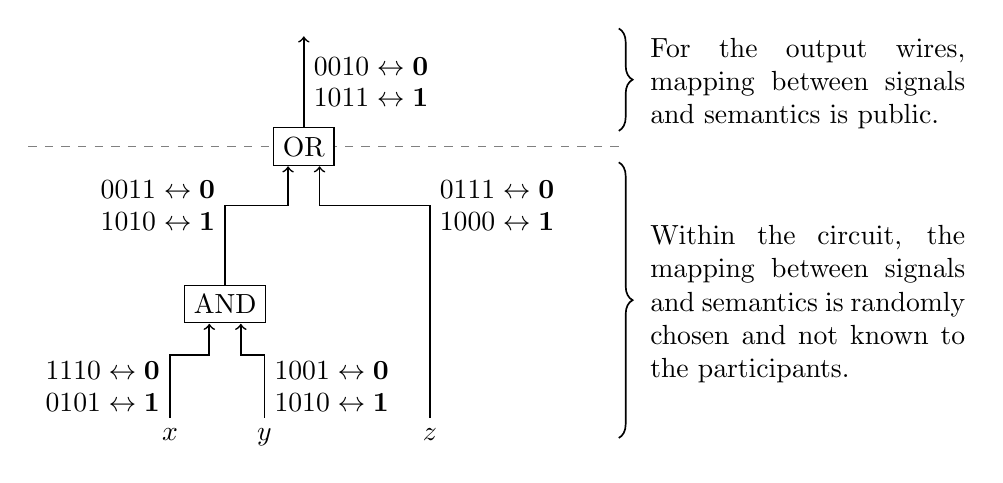
\begin{tikzpicture}
    \node (AND) at (0,1) [rectangle,draw=black] {AND};
    \node (OR) at (1,3) [rectangle,draw=black] {OR};
    % x->AND
    \draw[<-,semithick] (-.2,.75) |- +(-.5,-.4) -- 
      node[yshift=2mm,left] {$1110\leftrightarrow \mathbf{0}$} 
      node[yshift=-2mm,left] {$0101\leftrightarrow \mathbf{1}$} 
    +(-.5,-1.2) node[below] {$x$};
    % y->AND
    \draw[<-,semithick] (.2,.75) |- +(+.3,-.4) -- 
      node[yshift=2mm,right] {$1001\leftrightarrow \mathbf{0}$} 
      node[yshift=-2mm,right] {$1010\leftrightarrow \mathbf{1}$} 
    +(+.3,-1.2) node[below] {$y$};
    % AND->OR
    \draw[<-,semithick] (.8,2.75) |- +(-.8,-.5) 
       node[yshift=2mm,left] {$0011\leftrightarrow \mathbf{0}$ }
       node[yshift=-2mm,left] {$1010\leftrightarrow \mathbf{1}$ } --
    (AND);
    % z->OR
    \draw[<-,semithick] (1.2,2.75) |- ++(+1.4,-.5) 
      node[yshift=2mm,right] {$0111\leftrightarrow \mathbf{0}$} 
      node[yshift=-2mm,right] {$1000\leftrightarrow \mathbf{1}$} --
    +(0,-2.7) node[below] {$z$};
    % OR->output
    \draw[->,semithick] (OR) -- 
      node[yshift=2mm,right] {$0010\leftrightarrow \mathbf{0}$} 
      node[yshift=-2mm,right] {$1011\leftrightarrow \mathbf{1}$} 
    +(0,1.4);
    % legend
    \draw[dashed,gray](-2.5,3) -- (0.6,3);
    \draw[dashed,gray](5,3) -- (1.4,3);
    \draw[decoration={brace,amplitude=0.5em},decorate,semithick] (5,4.5)--(5,3.2);
    \draw[decoration={brace,amplitude=0.5em},decorate,semithick] (5,2.8)--(5,-.7);
    \node[text width=4cm,text justified] () at (7.4,1) {
      Within the circuit, the mapping
      between signals and semantics is
      randomly chosen and not
      known to the participants.};
    \node[text width=4cm,text justified] () at (7.4,3.8) {
      For the output wires, mapping between signals and semantics is public.
    };
  \end{tikzpicture}
  \caption{Associating random signals with semantics. The input wire for variable $y$ associates signal $1001$ with semantics $\mathbf{0}$ and signal $1010$ with semantics $\mathbf{1}$. While all input and internal signals and semantics can not be mapped onto each other, the signals and semantics of the \emph{output} wire are constructed in such a way that the signal's last bit coincides with the desired semantics. Note that the ``structure'' (i.e. placement of gates and wires) of the garbled circuit corresponds to that of the original circuit depicted in Figure \ref{fig:simple-circuit}.}
  \label{fig:associating-random-signals-with-actual-semantics}
\end{figure}

We come now back to our circuit $C$ and ``install the new signals'': Therefore, we ``remove the original signals'', and replace them by new (random) signals that are mapped onto semantics. We illustrate this concept in Figure \ref{fig:associating-random-signals-with-actual-semantics}. In our example, we see, that if the left incoming wire of the AND-gate holds signal 0101 (representing semantics \textbf{1}), and if the right incoming wire of the AND-gate holds 1001 (representing semantics \textbf{0}), we should get the ouput signal 0011 (representing semantics $\mathbf{0}=\mathbf{1}\wedge \mathbf{0}$).

Only the output wire's association between semantics and signals (i.e. $0010\leftrightarrow \mathbf{0}$ and $1011\leftrightarrow \mathbf{1}$) is publicly known. They are constructed such that the last digit of the signal corresponds to the desired semantics. This is useful since we want all participants to simply be able to deduce the functions outcome from the output wires of the circuit.

All \emph{internal} mappings from signals to semantics, are unknown to the participants. Please note the difference between the fact that the relation between internal signals and semantics is properly \emph{defined}, and the fact that they are \emph{not known} to the players. This is a central point for the protocol to work.

\paragraph{In a nutshell: What is our goal?}

We later want something like the following: Each player shall get the garbled circuit, and \emph{only} the input signals (also in garbled format). From these, each player shall be able to compute the output values of the circuit. This is depicted in figure \ref{fig:sample-computation}. On the way to this, the player shall not be able to deduce the semantics of input or intermediate wires\footnote{If some player supplies some input, she of course knows the semantics of the corresponding input wire. We just want to ensure that no player learns the semantics of inputs that are not supplied by herself.}.

Moreover, if a player has computed e.g. the even signal for a wire, she should not be able to deduce the odd signal for that wire.

\begin{figure}[t]
  \centering
  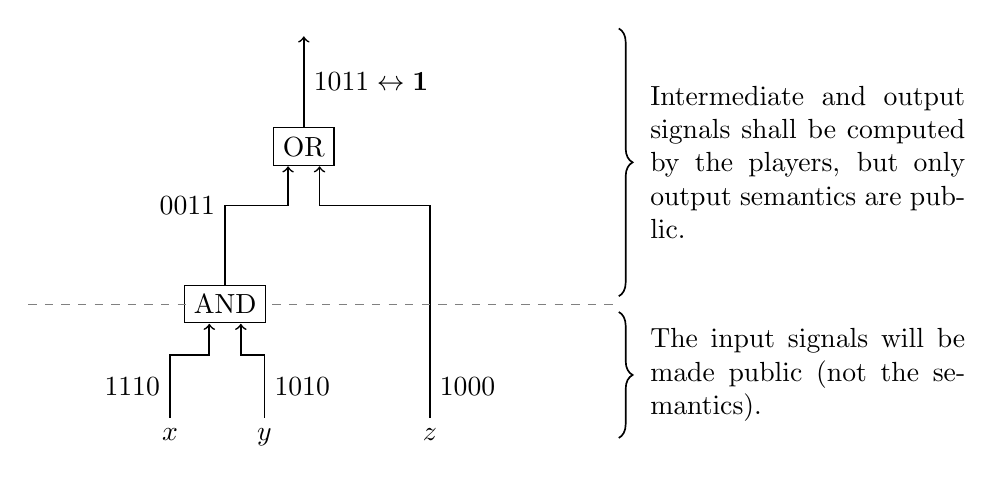
\begin{tikzpicture}
    \node (AND) at (0,1) [rectangle,draw=black] {AND};
    \node (OR) at (1,3) [rectangle,draw=black] {OR};
    % x->AND
    \draw[<-,semithick] (-.2,.75) |- +(-.5,-.4) -- 
      node[left] {$1110$} 
    +(-.5,-1.2) node[below] {$x$};
    % y->AND
    \draw[<-,semithick] (.2,.75) |- +(+.3,-.4) -- 
      node[right] {$1010$} 
    +(+.3,-1.2) node[below] {$y$};
    % AND->OR
    \draw[<-,semithick] (.8,2.75) |- +(-.8,-.5) 
       node[left] {$0011$ } --
    (AND);
    % z->OR
    \draw[<-,semithick] (1.2,2.75) |- ++(+1.4,-.5) 
      node[yshift=-2.3cm,right] {$1000$} --
    +(0,-2.7) node[below] {$z$};
    % OR->output
    \draw[->,semithick] (OR) -- 
      node[right] {$1011\leftrightarrow \mathbf{1}$} 
    +(0,1.4);
    % legend
    \draw[dashed,gray](-2.5,1) -- (-.5,1);
    \draw[dashed,gray](.6,1) -- (5,1);
    \draw[decoration={brace,amplitude=0.5em},decorate,semithick] (5,4.5)--(5,1.1);
    \draw[decoration={brace,amplitude=0.5em},decorate,semithick] (5,.9)--(5,-.7);
    \node[text width=4cm,text justified] () at (7.4,.1) {
      The input signals will be made public (not the semantics).
      };
    \node[text width=4cm,text justified] () at (7.4,2.8) {
      Intermediate and output signals shall be computed by the players, 
      but only output semantics are public.
    };
  \end{tikzpicture}
  \caption{Our goal: The players shall -- given a garbled circuit and garbled inputs -- compute intermediate and output signals. From the output signals, they can deduce the output of the function. This example shows the garbled inputs for $x=\mathbf{0}, y=\mathbf{1}, z=\mathbf{1}$ (see figure \ref{fig:associating-random-signals-with-actual-semantics} for reference). The players shall not be able to deduce the other signals for the wires. Since $f(0,1,1) = (0\wedge 1) \vee 1 = 1$, each player shall -- at last -- learn the output signal $1011$ which stands for semantics $\mathbf{1}$.}
  \label{fig:sample-computation}
\end{figure}


\paragraph{Format of the signals.}

Note that all signals have the same length and are binary strings. Moreover, it is worth noting that for each wire, exactly one signal is ending in 1, while the other is ending in 0. We call the signals ending in 0 ``even signals'' and the signals ending in 1 ``odd signals'' (for obvious reasons). Even if we don't strictly need this convention, it is quite helpful and makes notational issues a bit easier.

Since we want to collaboratively compute the circuit, it should not be the case that e.g. one single player has to define all the signals, and possibly declare his defined signal public. We rather choose some method where all signals are composed of parts supplied by \emph{all} participating parties. To be precise, we require that each party contributes $k$ bits to each signal ($k$ denoting the security parameter). Moreover, we want to construct the signals randomly, since we wanted that concluding the semantics from a signal is not possible (for internal and input wires).

If each of the $n$ players contributes $k$ bits, these are $nk$ bits. To these bits, we add one single bit (again collaborytively randomly chosen) indicating whether it is the even or odd signal (the so-called \emph{parity}). These, in turn, makes signals of length $nk+1$.

Having this construction in mind, we can interpret a signal (i.e. a bit string) of length $nk+1$ as a concatenation of $n$ bit strings each having length $k$ and one last bit to determine whether the signal is odd or even.

So, the only remaining (but very central) question is: ``How can we assure that the intermediate values (i.e. the internal signals) are computed correctly, even if we don't know the association between signals and semantics?''

\paragraph{How can signals propagate along the gates?}
\label{sec:how-can-signals-propagate}

In order to compute the final output value, we will have to determine the output wire's signal (and -- since for this wire we know the mapping -- its semantics). Therefore, we have to compute internal signals along the wires.

To do this, we employ an auxiliary table for each single gate that helps us computing the gate's functionality. We denote the gate's functionality by the symbol $\otimes$ (i.e. the symbol $\otimes$ represents e.g. OR, AND, XOR, NAND or another binary function on bits). This auxiliary table holds four (binary) strings, each of which has length equal to the length of the signals. We construct these bit strings for each gate $g$ and call them call them $A_{00}^g,A_{01}^g,A_{10}^g$ and $A_{11}^g$ (we use superscript $g$ to specify the gates for which the strings are used). 

So, we get a table consisting of 4 rows for a gate taking two inputs and having one output. Remember that we assumed our circuit consisting only of gates with two inputs. Since each input wire can carry either an odd or an even signal, that makes 4 possibilities for the input semantics in total.

As you might guess, that every single entry of these 4 entries in the table is used for one specific computation of the gate, i.e. for one specific combination of odd and even signals along the input wires. For example, if the two input wires of gate $g$ are even, we have to use $A_{00}^g$. If the left incoming wire of gate $g$ carries an odd signal, and the right incoming of gate $g$ carries an even signal, we have to use $A_{01}^g$ for the computation. That is, one has to consider the last bits of the signals carried by the two incoming wires, and choose the value from the table accordingly.

But what do the values of this table ($A^g_{00},A^g_{01},A^g_{10}$ and $A^g_{11}$) look like? Note that we said that the length of a signal is $nk+1$. In order to understand how the table works, we interpret a single signal as $n$ strings, each of length $k$, i.e. we split up the signal into several pieces. Note that, since the length of a signal was $nk+1$, we discard the last bit when doing so.

As we mentioned before, we consider one signal (of length $nk+1$) as $n$ binary strings of length $k$ and one additinal parity bit (telling us whether the signal is odd or even). We now split up an incoming signal into $n$ strings of length $k$ and issue each of these strings as input to a pseudorandom generator $G$. This pseudorandom generator (taking a string of length $k$) stretches this input into a longer (binary) string (of length equal to the length of one single garbled signal). This longer string is then split up into two halves that we call $G_0(s)$ and $G_1(s)$ (for the ``zeroth'' and the ``first'' half of the generator's output).

%Each of these pieces is then used as an input for a pseudorandom generator. Such a generator $G$ shall take $k$ input bits (since each piece consists of $k$ bits), and should produce an output of $2(\overline{n}k+1)$ bits, where $\overline n = k^{10}$ (arbitrary).\todo{Genauer auf $\overline n$ eingehen.} We then take the pseudorandom generator's output $G(s)$ and split it into two bit strings of length $\overline n k + 1$. We call these two bit strings $G_0'(s)$ and $G_1'(s)$, respectively.\todo{Formalize this and make a picture.} From these two strings of length $\overline n k$, we take the first $nk+1$ bits to obtain $G_0(s)$ and $G_1(s)$, respectively.

Depenging on the parity on the incoming signal, we either use $G_0$ or $G_1$. If the incoming signal is even, we use $G_0$, while we use $G_1$ if the incoming signal is odd. That is, we split up the signal into $n$ bit strings, feed each of them into a random generator and use the respective halves of the outputs generated by the calls to our random generator $G$. We will come back to that later in more detail (i.e. we will explain how long the output of $G$ is exactly, and which pieces exactly are given to $G$ as inputs). 

That essentially means: For a given even signal (i.e. a signal ending in 0), we compute $G_0(s)$ for all pieces $s$ obtained by splitting up the signal. We proceed analogue for odd signals.

%If an input wire for a gate carries an odd signal (i.e. a signal ending in 0), we compute $G_0(p)$ for all pieces $p$ obtained by splitting up the signal (except the last bit) into $n$ bit strings of length $k$. On the other hand, if the wire holds an odd signal, we compute $G_1(p)$ for all pieces $p$. That is, like the input signals determined which table entry to use, we also use these input signals to choose the correct pseudorandom generator.

We take then the bitwise exclusive-or (XOR) of all the values obtained by the pseudorandom generators and the appropriate table entry.

So, let us for now assume that we are considering -- for a certain gate -- the following input signals (for left and right input wire, respectively):

\begin{equation*}
  \sigma=\sigma_1\dots\sigma_na  \quad \text{ and }\quad \tau=\tau_1\dots\tau_nb.
\end{equation*}

That is, each $\sigma_i$ is a bit string of length $k$ and the signal $\sigma$ has parity $a$. Analogously the input signal $\tau$ consists of $n$ parts having length $k$ each (the single $\tau_i$). Then, we later want to be able to compute the gate's output as follows:

\begin{equation}
\label{eq:definition-of-output-of-a-gate-dependent-of-gate-label}
  output \gets G_b(\sigma_1)\oplus\dots\oplus G_b(\sigma_n) \ \oplus \ G_a(\tau_1)\oplus\dots\oplus G_a(\tau_n) \ \oplus \ A_{ab}^g
\end{equation}

You can treat the arrow-sign ($\gets$) as an equality sign. We just chose this symbol here, because we wanted to emphasize that the output \emph{is computed} from some other values. That is, we have to consider all input signals (i.e. all combinations of odd/even signals for this gate) and compute the corresponding table entry $A_{ab}^g$

Let us now think for a moment, why we exactly want to define the output like this: 

In the above equation, $output$ denotes the proper desired result for the specific gate. It should be no too hard problem to solve the above equation (resp. definition) for $A_{ab}^g$ (remark: $a$ and $b$ were the parities of the input signals $\sigma$ and $\tau$, respectively). 

If we do so, we can derive how to construct the values $A_{00}^g,A_{01}^g,A_{10}^g$ and $A_{11}^g$ (by substituting $a$ and $b$ by appropriate values). We now solve equation (\ref{eq:definition-of-output-of-a-gate-dependent-of-gate-label}) for $A_{ab}^g$:

\begin{equation}
  \label{eq:gate-label-definition-with-output}
  A_{ab}^g = G_b(\sigma_1)\oplus\dots\oplus G_b(\sigma_n) \ \oplus \ G_a(\tau_1)\oplus\dots\oplus G_a(\tau_n) \ \oplus \ output
\end{equation}

Even if this beast doesn't look that nice to us (and even if we didn't specify the term $output$ exactly in the above equation), we already now see the following: Equation (\ref{eq:gate-label-definition-with-output}) consists essentially of terms obtained by a random generator (these are the terms $G_b(\sigma_i)$ and $G_a(\tau_j)$) and one term $output$ that are XORed to obtain the result $A_{ab}$. Remember: In section \ref{sec:building-blocks-for-the-protocol} we talked about collaboratively evaluating the XOR-function. We said that we can do this in a constant number of rounds with polynomial amount communication. That means: If we know how to compute the term $output$, we can evaluate this huge XOR in a constant number of rounds with only communication only.

What you should recognize is the following: Equation (\ref{eq:gate-label-definition-with-output}) seems to contain no parametrization that ``adjusts'' the value $A_{ab}$ to the kind of gate that value will later be used for. This information is contained in the term $output$. Let us now see, what this term is looks like exactly.

Therefore, remember that the term $output$ should contain the result that one gets when evaluating the considered gate with inputs $\sigma$ and $\tau$, respectively. To be a bit more precise, $output$ shall represent the signal that is ``returned'' by the gate for the given inputs.

Remember that we assigned signals \emph{to each wire}, i.e. in particular to the output wire of the gate we're considering. Moreover, the left input wire holds the signal $\sigma_a$ (i.e. a signal with parity $a$) and the right input wire holds the signal $\tau_b$ (i.e. a signal with parity $b$). As we stated before, for each wire, each of the two signals represents exactly one semantic ($\mathbf{0}$ or $\mathbf{1}$). We now want the following: We want to determine the correct outgoing signal such that the \emph{semantics} associated with the computed outgoing signal are the same as the \emph{semantics} we would obtain if we would map $\sigma_a$ and $\tau_b$ onto their respective semantics and evaluate the ungarbled (i.e. the original) gate for these input semantics. That is we essentially want to know: ``What would the original gate return on inputs represented by the semantics of the input wires?'' The obvious problem here is of course, that we do not know the mapping between signals and semantics, and we just have the signals.

Surprisingly, it is still possible to properly compute the outgoing signal such that its associated semantics represent the desired computation! 

\paragraph{How to compute the value of the variable $output$.}
\label{sec:how-compute-value-variable-output}

Before we go on, we need some additional definitions. First of all, let us give names to these wires: We call the input wires $\alpha$ and $\beta$ (carrying signals $\sigma$ and $\tau$, respectively), and we call the outgoing wire $\gamma$ (will then carry the signal we want to compute).

Let us call the even and odd signals for the gate's output wire $s^\gamma_0$ and $s^\gamma_1$, respectively (remember: these are just signals, and we do not know the mapping to the associated semantics). That is, when we want to compute the gate's output, we have to decide whether we choose $s^\gamma_0$ or $s^\gamma_1$ as the resulting signal. So, essentially, we have to compute the subscript index.

\newcommand{\semoutput}{\lambda}

Moreover, we will need the \emph{semantics} for the incoming wires and outgoing wire. 

We will now need a single bit for each of these three wires -- for now called $\semoutput_\alpha,\semoutput_\beta,\semoutput_\gamma\in\left\{ 0,1 \right\}$ -- that defines for the corresponding wire whether the even signal is associated with semantics $\mathbf{0}$ or vice versa. The subscript denotes the wire that is associated with that bit.

That is, if e.g. $\semoutput_\alpha=0$ (this bit is of course for wire $\alpha$), we -- on this wire -- associate the even signal with semantics $\mathbf{0}$ and the odd signal with $\mathbf{1}$. If $\semoutput_\alpha=1$, it is just the other way around\footnote{The bit $\semoutput$ basically tells us how we can construct the semantics from the last bit of the outgoing signal.}. As you can see, one single bit suffices to fully define the semantics of a wire.

Note that using this bit, one can easily compute the semantics from a signal (for a specific wire). We simply take the last bit of the signal (the parity bit) and XOR it with the corresponding bit $\semoutput$ for this wire.

% Even if we introduced $\semoutput$ just for the output wire (since we are for now just interested in how to evaluate a gate), we will later need such a bit for \emph{each single wire} (so that the mapping between signals and semantics is defined for each wire).

\begin{equation}
  \label{eq:output-straight-definition-in-informal-part}
  output := s^\gamma_{ \left[ (\semoutput_\alpha \oplus a) \otimes (\semoutput_\beta \oplus b)\right]  \oplus \semoutput_\gamma}
\end{equation}

So, why does this make sense? Consider for now, just the subscript index
\begin{equation*}
\left[ (\semoutput_\alpha \oplus a) \otimes (\semoutput_\beta \oplus b)\right]  \oplus \semoutput_\gamma
\end{equation*}
and take it to pieces:

The term $(\semoutput_\alpha \oplus a)$ is the \emph{semantics} carried by the input wire $\alpha$ (we said that we can compute the semantics by taking the XOR of the $\semoutput$-variable with appropriate index -- in this case $\alpha$ -- and the parity bit, which is -- in this case -- $a$). Analogously, $(\semoutput_\beta \oplus b)$ is the semantics carried by input wire $\beta$.

Remember that we are considering one particular gate that computes the function denoted by the symbol $\otimes$. Thus, $(\semoutput_\alpha \oplus a)\otimes (\semoutput_\beta \oplus b)$ is exactly the semantics that we expect to obtain on wire $\gamma$ when we would evaluate the original gate. Thus, if we want to have the associated signal to that semantics, we have to reconstruct it by XORing this value with $\semoutput_\gamma$.

That is, if we define $output$ this way, it gives us \emph{exactly} the signal we need for the output wire.

Moreover note that we said that it is possible to evaluate a circuit with bounded fan in and depth $d$ in $O(d)$ rounds with polynomial communication. Note that the circuit needed to compute this subscript has bounded fan-in and constant depth, thus can be computed in $O(1)$ rounds.

It remains to clear how the values $\semoutput_\alpha,\semoutput_\beta$ and $\semoutput_\gamma$ are constructed. Again, since we do not want any participant to compute something alone, we construct these values collaboratively. Therefore, the participants generate random bits and take the XOR of them. Again, this is a collaborative evaluation of the XOR function which -- as we know -- can be evaluated in a constant number of rounds with polynomial communication amount.

But when one considers equation (\ref{eq:gate-label-definition-with-output}), one might ask, why we XOR this value with all the outputs generated by some pseudorandom generators. This is exactly what prevents all participants from determining the mapping between signals and semantics: If we generate the gate labels using pseudorandom generators, no one can conclude the mapping between signals and semantics, since it is scrambled (for a bit more on this, please consult section \ref{sec:appendix-why-pseudorandom-generators}). 

So far, we have seen how we can compute the output \emph{signal} of a certain gate, given its input signals (not its input \emph{semantics}). That way, we can ``go through'' the circuit and evaluate one gate after another, finally arriving at the gates whose outgoing wires represent the functions output value.

If we now want to compute our original function, we can just evaluate the circuit associated with proper inputs. Since the mappings from from signals to semantics are known for the output wires, we can reconstruct the solution representing our function value.

\section{A (more) formal depiction of the protocol}
\label{sec:formal-description}

We saw in section \ref{sec:concrete-idea} how we can transform any function (represented as a circuit) into a garbled circuit that can be used later to evaluate the function given certain inputs. We will now give a formal summary that explains how to construct a garbled circuit and how to evaluate it locally. This steps are in principle taken from \cite{Rogaway:1991:RCS:888502}, with some explanations added. 

The protocol itself has two main steps. First, the participants \emph{collaboratively} construct the garbled circuit needed for our function. In the second step, the participants \emph{locally} do the (expensive) evaluation of the garbled circuit. But before we start with the actual construction, we have to ensure that the circuit we are starting with has a certain format. We will now discuss all these aspects in more detail.

\subsection{Bringing the original circuit into a suitable format}
\label{sec:original-circuit-suitable-format}

We already mentioned in section \ref{sec:general-idea} that we can assume the circuit in a suitable format. We briefly recapitulate how the circuit should look like: It should have no ``circles'', only gates with a fan-in/fan-out combination of $2/1$ or $1/2$. It is a well known fact that each circuit can be represented using only such gates without increasing the circuit's size too much (i.e. the size stays polynomial).

\subsubsection{Introducing ``splitters''.}
\label{sec:introducing-splitters}

As we will discuss later (and as it was shown roughly ten years after the protocols initial publication by \cite{Tate03ongarbled}), we have to require the following for our circuit: No wire is used more than once as an input wire.

To be able to ensure this, we need so-called \emph{splitter} gates that take one signal as input and have two outgoing wires. The incoming signal is then just forwarded to each of the outgoing wires. While this might seem just to be a complication of matters, we will later inspect why this is necessary.

That is, whenever one input wire is used as input to more than one gate, we use splitters to split up the signal onto several distinct wires. Again, note that this doesn't increase the size of the circuit more than by a polynomial factor.

Keep in mind that our circuit $C$ has now two kinds of gates: Gates taking two inputs and returning one output (the ``ordinary gates''), and gates taking one input and returning two outputs (the splitters we had to introduce).

\subsection{Constructing the garbled circuit}
\label{sec:protocol-construct-garbled-circuit}

In order to understand how the protocol works, let us first consider the inputs to our problem:

\begin{description}
\item[Common input.] The common input can be seen as a string:

  \begin{equation*}
    c=1^{k'}\#1^n\#1^\ell\#1^l
    % \#m % brauchts nicht unbedingt
    \#C
  \end{equation*}

This string is basically just used so that all participants know ``what's going on''. The parameter $k'$ defines a lower bound for the security parameter (see below how we obtain the actual security parameter $k$ from $k'$), while $n$ is the number of participants, $\ell$ stands for the length of one party's input\footnote{We assume all inputs from the parties to be of equal length.} and $l$ is the length of the output value.

That is, we -- formally -- consider a function $f:(\Sigma^\ell)^n\rightarrow \Sigma^l$ accepting $n$ inputs of length $\ell$ and returning one value of length $l$. We could assume simpler sets here, but we chose to use these to be consistent with \cite{Rogaway:1991:RCS:888502}. $C$ is a suitable circuit-representation of the function $f$. 

%\todo{Wofür brauchts $m$?}

\item[Private inputs.] Each participating party $i$ has a private input $x_i\in\Sigma ^\ell$ that shall not become known to other participants.
\end{description}

\subsubsection{Computing gate labels and semantics.}
\label{sec:gate-labels-and-semantics-formal-def}

Let us in the following assume that $C$ has $\Gamma$ gates (numbered $1,2,\dots,\Gamma$) and $W$ wires (numbered $1,2,\dots,W$, including input, internal and output wires). The input wires are the wires $1,2,\dots,n\ell$, output wires are assigned the numbers $W-l+1,W-l+2,\dots W$.

What we will now do is computing the garbled circuit. That is, we will collaboratively compute gate labels for each gate and we will compute the semantics for each wire. Remember that it is crucial to keep the semantics secret so no participant can conclude the ``real values'' along the wires, but just sees the signals. Moreover, we will later just ``publish'' the correct signals for the input wires and the gate labels. We will compute these values collaboratively and randomly.

We remember that we needed four gate labels for each gate\footnote{A ``normal gate'' needs four gate labels, because it has exactly two input wires that can carry even or odd signals each. 

A splitter gate needs four labels as well, since it has one input and two outputs. Thus, the input signal can be even or odd, and we need these two possibilities for each of the two outgoing wires.}. Moreover, we said that each player shall contribute $k$ bits to each signal. Be careful here: Each player has to generate $k$ bits for every wire \emph{for the even and for the odd signal}. Additionally, we stated that we wanted all players to contribute one bit to the semantics $\lambda^\omega$ for some wire $\omega$. That means, each player $i$ has to generate a random bit string $r_i\in\Sigma^{2kW+W-l}$ ($W$ is the number of wires in total).

The strings $r_i$ will later be interpreted in the following way:

\begin{equation}
  \label{eq:interpretation-random-string-of-a-player}
  r_i=s_{0,i}^1,s_{1,i}^1,\dots,s_{0,i}^W,s_{1,i}^W,\  \lambda_i^1,\dots,\lambda_i^{W-l}
\end{equation}

Each string $s^\omega_{p,i}$ is then a random bit string of length $k$ generated by player $i$ that ``participates'' in the parity-$p$-signal for wire $\omega$ (and thus, implicitly in the gate labels). The value $\lambda_i^\omega$ is some bit that will later ``participate'' in the \emph{semantics}\footnote{Remember that we stated that if $\lambda^\omega=0$ then the even signal is associated with semantics $\mathbf{0}$ and the odd signal is associated with semantics $\mathbf{1}$. If $\lambda^\omega=1$, it is just the other way around.} of wire $\omega$. See below how this is to be understood. Note that we do only need $\lambda_i^1,\dots,\lambda_i^{W-l}$ since we wanted the semantics of the $l$ output wires to be public.

%The parties' aim is to compute so-called \emph{gate labels} $A^g_{00}, A^g_{01}, A^g_{10}, A^g_{11}$ and input signals $\sigma^\omega\in\Sigma^{nk+1}$ for $g\in \left\{1,2,\dots,\Gamma \right\}$ and for $\omega\in\left\{1,2,\dots,n\ell \right\}$, where $\Gamma$ denotes the number of input wires to the circuit.

Let now the actual security parameter $k=\max(k',\sqrt[10]{|c|})$. This is a technical detail that is necessary due to our definition of adversaries. These adversaries are allowed to use polynomial time in $|c|$, and not in $k$. For more information please consult \cite{Rogaway:1991:RCS:888502}.

Now, the parties compute gate labels and input signals with security parameter $k$ -- tolerating the presence of at most $\lfloor \left( n-1 \right) / 2\rfloor$ adversaries (speak: they ``\emph{information-theo\-retically} $\lfloor (n-1)/2 \rfloor$-securely'' compute all this) using the following technique:

\paragraph{Private inputs.}

The private inputs $x_1,\dots,x_n$ define the bits $b^1,\dots,b^{n\ell}$ associated with each input wire, according to $b^1\dots b^{n\ell}=x_1\dots x_n$. Each $x_i$ supplies $l$ bits (namely $b^{(i-1)\ell+1}$ to $b^{i\ell}$).

\paragraph{Defining the signals.}

We now define for each wire $\omega\in\left\{ 0,\dots,W \right\}$ and for each parity $b\in\left\{ 0,1 \right\}$ the signals:

\begin{equation}
  \label{eq:definition-of-signals}
  s_b^\omega:=s_{b,1}^\omega\dots s_{b,n}^\omega b
\end{equation}

This means, for $b=0$ we have the even signals, while $b=1$ gives an odd signal. Note that only the input signals (representing the correct semantics) can later be revealed to the public safely. But remember: We won't publish the semantics!

\paragraph{The semantics of the wires.}

We come now to a central part of this construction: We define the semantics of each wire $\omega$.

\begin{equation}
  \label{eq:definition-of-semantics-formal}
  \lambda^\omega= 
  \begin{cases}
    \lambda_{1}^\omega\oplus\dots\oplus\lambda_{n}^\omega & \text{ for } 1\leq\omega\leq W-l \\
    0 & \text{ for } W-l+1\leq\omega\leq W.
  \end{cases}
\end{equation}

Please note that equation (\ref{eq:definition-of-semantics-formal}) contains just a \emph{definition}. It is important that neither $\lambda^\omega$ nor $\lambda_i^\omega$ become public. We define a notational shorcut: We say that $\lambda^\omega$ is the semantics of signal $s_0^\omega$, while $\overline{\lambda^\omega}:=1-\lambda^\omega$ is the semantics of signal $s_1^\omega$.

\paragraph{Signals along input wires.}

For each input wire $\omega$ of the circuit (i.e. for each $\omega \in \left\{ 1,2,\dots,n\ell\right\})$, the string $\sigma^\omega$ is given by
  \begin{equation}
    \label{eq:sigma-superscript-omega-definition}
    \sigma^\omega=s_{(b^\omega\oplus\lambda^\omega)}^\omega.
  \end{equation}

To research what $\sigma^\omega$ means, we assume we have an input wire (in the sense that it is an input wire to the whole circuit) $\omega\in\left\{ 1,2,\dots,n\ell \right\}$ that has semantics $\lambda^\omega$. Then, the subscript $(b^\omega\oplus\lambda^\omega)$ denotes the parity that is needed for this particular input wire to correctly represent the semantics of the player's input. If we then take $s_{(b^\omega\oplus\lambda^\omega)}^\omega$, we can be sure that we are issuing the correct input signal (one can simply test this with sample values for $b^\omega$ and $\lambda^\omega$).

Note that even if the original input signal comes from one single player, the computation of $s_{(b^\omega\oplus\lambda^\omega)}^\omega$ has to be done collaboratively, since it involves $\lambda^\omega$ (the semantics for wire $\omega$) that shall not become public and since signals are composed of bits supplied by all players. However, that collaborative computation is no problem, since se already saw that we can compute the subscript
\begin{equation}
\label{eq:computing-input-signals}
(b^\omega\oplus\lambda^\omega)\stackrel{~(\ref{eq:definition-of-semantics-formal})}{=}(b^\omega\oplus\lambda_{1}^\omega\oplus\dots\oplus\lambda_{n}^\omega)
\end{equation}
is, as we see, essentially just a XOR of bits, whose associated circuit can be secretly and securely evaluated in a constant number of rounds and with polynomial communication.

In this way, all players learn the value $\sigma^\omega$ without learning the value $b^\omega$ (which shall stay private to the player holding it). The players then only compute the signal associated with the obtained parity. This way, only this signal is learnt by all players.

\paragraph{Constructing the gate labels.}

It remains to explain how we can -- given the input signal(s)\footnote{Again without knowing the input \emph{semantics}.} to a gate $g$ -- later be able to compute the output of this certain gate. Therefore, we define the gate labels (as explained in section \ref{sec:signals-semantics-by-example}). 

We assume now that $\alpha, \beta$ denote input wires carrying signals $\sigma^\alpha_a$ and $\sigma^\beta_b$, respectively. The signals have the following format:

\begin{equation*}
  \sigma^\alpha_a=s_{a1}^\alpha\dots s_{an}^\alpha a  \quad \text{ and }\quad \sigma^\beta_b=s_{b1}^\beta\dots s_{bn}^\beta b
\end{equation*}

This means: On wire $\alpha$, there's the signal with parity $a$ for that specific wire, consisting of the $n$ sub-strings $s_{ai}^\alpha$ of length $k$ each, and with the parity bit $a$. We have the corresponding parts for $\sigma_b^\beta$.

Remember: We have two kinds of gates in our circuit: The ``ordinary gates'' taking two inputs and returning one output and the ``splitters'' taking one input and having two output wires.

\begin{description}
\item[``Ordinary gates''.] We will start with the ``ordinary gates''. These gates get two input signals and return one output signal. For each ordinary gate $g$ in the circuit (i.e. $g$ is some number in $\left\{ 1,2,\dots;\Gamma \right\}$), we define the gate labels $A^g_{00}, A^g_{01}, A^g_{10}, A^g_{11}$ as follows: If gate $g$ computes a binary function we denote by the symbol $\otimes$, and has left wire $\alpha$, right wire $\beta$, and output wire $\gamma$ (i.e. $\alpha,\beta,\gamma\in[1\dots W]$), then we define for $a,b\in\{0,1\}$ the gate label $A_{ab}^g$ by
  \begin{eqnarray*}
    A_{ab}^g &= & G_b(s_{a1}^\alpha)\oplus\dots\oplus G_b(s_{an}^\alpha) 
              \ \oplus \ 
              G_a(s_{b1}^\beta)\oplus\dots\oplus G_a(s_{bn}^\beta)
              \ \oplus \ \\
             & & s_{[(\lambda^\alpha\oplus a)\otimes(\lambda^\beta\oplus b)]\oplus\lambda^\gamma}^\gamma
  \end{eqnarray*}
\item[Splitter gates.] We will now do the analogue thing for splitter gates. Even if we didn't specify these gates in section \ref{sec:how-can-signals-propagate}, the underlying thoughts are the same. Remember that a splitter just forwards its input signal onto the two outgoing wires. We call the single input wire $\alpha$ and denote the output wires by $\gamma_0$ and $\gamma_1$. Then, the gate labels are as follows (for $a,b\in\left\{ 0,1 \right\}$):
  \begin{eqnarray*}
    A_{ab}^g & = & G_a(s^\alpha_{a,1}) \oplus \dots \oplus G_a(s^\alpha_{b,n}) \oplus s^\alpha_{(\lambda^\alpha\oplus b)\oplus\lambda^{\gamma_a}}
  \end{eqnarray*}
\end{description}
\todo{Gate labels für splitter nochmal checken!}

As said before, $G_0$ and $G_1$ denote the ``zeroth'' and the ``first'' halves of the output of a pseudorandom generator $G$. This pseudorandom generator takes a binary string of length $k$ ($k$ being the security parameter) and stretches it into a longer string. The length of this longer string has to be fixed a priori, which is why we assume that the generator returns a binary string of length $2(\overline{n}k+1)+1$, with e.g. $\overline{n}=k^{10}$. The term $\overline{n}$ bounds the number of players that can participate in the protocol depending on the security parameter. Thus, $\overline{n}=k^{10}$ shouldn't be a too hard restriction, but can be increased at will (at least as long as it is a fixed power of $k$). For the reasoning why we define $A^g_{ab}$ exactly like that, please refer to section \ref{sec:how-can-signals-propagate}.

\paragraph{Outcome of the first phase of the protocol.}

We have computed two important things in common: The whole garbled circuit (consisting of gate labels and associated wires) and the input signals ($\sigma^\omega$ for $\omega\in\left\{ 1,2,\dots,n\ell \right\}$).

The semantics ($\lambda^\omega$ for $\omega\in\left\{ 1,2,\dots,W-l+1 \right\}$) are \emph{not known} to the participants. It is crucial that this is the case since otherwise the players could deduce e.g. the input values and internal values of wires. It is all the more surprising that we can evaluate the function correctly, even if we don't know the internal wires values.

What we've done now is the following: The parties collaboratively computed the garbled circuit (with security parameter $k$, and $\lfloor (n-1)/2 \rfloor$-securely). Note that we didn't exactly specify how e.g. the several XOR-operations are computed collaboratively, but we just said that \emph{we are using} some techniques that enables us to do so. We saw in section \ref{sec:building-blocks-for-the-protocol} that such a protocol for XOR exists.

In this way, we can rely upon the existing protocols that serve as building blocks for our protocol. Moreover, this takes the burden of some proofs from us: We just know that there exist some protocols that we can use as building blocks for our protocol, and if these building blocks have specific properties, they automatically apply for our protocol. 

In particular, we saw that every step described could be evaluated in a constant number of rounds and with polynomial overhead. Since the first phase has no loops or recursions, the overall complexity is still within a constant number of rounds and polynomial amount of communication.

It remains now for the single parties to evaluate the obtained garbled circuit. This is done in the second phase.

\subsection{Locally evaluating the garbled circuit}
\label{sec:protocoll-locally-evaluating-garbled-circuit}

We saw in the previous section how to construct the garbled circuit and will now examine how to evaluate the garbled circuit we obtained by the above routine.

As before, take a first look at the inputs:

\begin{description}
\item[Common input] As before, we have a common string $c=1^{k'}\#1^n\#1^\ell\#1^l\#m\#C$. For the meanings of all the symbols, please consult section \ref{sec:protocol-construct-garbled-circuit}.
\item[Input] Now we have a garbled program $\hat y$, i.e. we have gate labels $A^g_{00}, A^g_{01}, A^g_{10}, A^g_{11}\in\Sigma^{nk+1}$ and input signals $\sigma^\omega\in\Sigma^{nk+1}$ (for $g\in[1\dots\Gamma]$ and $\omega\in[1\dots nl]$).
\end{description}

We want to compute the string $y\in\Sigma^l$ that this garbled program evaluates to. As in the previous step, we set $k=max(k',\sqrt[10]{|c|})$. It is necessary for a player $i$ to know the value $k$, so that the player knows how to dissect a signal into $n$ binary strings of length $k$.

The following is carried out by each player $i$ (since we want to evaluate locally). That is, each player has to ``start at the input wires'' (using the values $\sigma^1$ to $\sigma^{n\ell}$) and work his way up to the output wires to evaluate the function.

We are now going to see how we can obtain the signals for the outgoing wires of the gates. Therefore, we again distinguish between ``ordinary'' and splitter gates:

\begin{description}
\item[``Ordinary gates''.] We consider how to evaluate an ordinary gate $g$ with left input wire $\alpha$, right input wire $\beta$ and output wire $\gamma$ (i.e. $\alpha,\beta,\gamma\in[1\dots W]$) given its input signals.

Let $\sigma^\alpha=\sigma_1^\alpha\dots\sigma_n^\alpha a$ be the signal for wire $\alpha$, and $\sigma^\beta=\sigma_1^\beta\dots\sigma_n^\beta b$ for wire $\beta$. Then, we want to compute the resulting signal $\sigma^\gamma$ for wire $\gamma$. Therefore we use the appropriate gate labels:

\begin{equation}
  \label{eq:player-i-holds-signal-definition}
  \sigma^\gamma=G_b(\sigma_1^{\alpha})\oplus\dots\oplus G_b(\sigma_n^{\alpha})
               \ \oplus \
               G_a(\sigma_1^{\beta})\oplus\dots\oplus G_a(\sigma_n^{\beta})
               \ \oplus\ 
               A_{ab}^g
\end{equation}

\item[Splitter gates.] Similarly, we compute the outgoing signal from a splitter gate. As we said, in splitter gates we only have one incoming signal, namely $\sigma^\alpha=\sigma_1^\alpha\dots\sigma_n^\alpha a$, and we have two outgoing wires $\gamma_0$ and $\gamma_1$ which we want to compute the signals for. That is, for $i\in\left\{ 0,1 \right\}$ we compute
  \begin{equation}
    \label{eq:splitter-gates-computation-of-output-values}
    \sigma^{\gamma_i}=G_i(\sigma_1^\alpha)\oplus\dots\oplus G_i(\sigma_n^\alpha) \ \oplus A_{ia}^g
  \end{equation}
\end{description}

\todo{Zeug für die Splitter gates nochmal genau checken.}

Please note that equation (\ref{eq:player-i-holds-signal-definition}) resembles equation (\ref{eq:definition-of-output-of-a-gate-dependent-of-gate-label}), which was the starting point of our thoughts when it came to how we would like to construct the gate labels. Equation (\ref{eq:splitter-gates-computation-of-output-values}) was derived in an analogue way.

So, we have seen how we compute the output of a certain gate. Thus, we can now ``propagate up the circuit'' and will reach the output wires. As soon as a player has computed a signal for each wire, she's basically done and can read the function output $y$:

\begin{equation}
  \label{eq:protocoll-each-player-ouputs}
  y=\lsb(\sigma^{W-l+1})\dots\lsb(\sigma^W)
\end{equation}

In equation (\ref{eq:protocoll-each-player-ouputs}), $\lsb$ denotes the least significant (in our case the last) bit. We can be sure that $\lsb(\sigma^{W-l+1})\dots\lsb(\sigma^W)$ is directly the output of the function, because we explicitly stated that the output wires ($W-l+1$ to $W$) have semantics that are publicly known (namely $\lambda^{W-l+1}=\dots=\lambda^W=0$).

\subsection{Review of the steps}
\label{sec:review-of-the-protocol}

\subsubsection{Ensure that the circuit has a certain format.}
\label{sec:ensure-that-circuit-has-a-certain-format}

Let us shortly recapitulate what we have done. We first ensured that the circuit representing the desired function has a certain format (no circles, only two-in-one-out- and one-in-two-out-gates, no wire used as input in more than one gate). It should be clear that transforming any circuit into a circuit satisfying these constraints can be done in polynomial time and moreover requires no communication between the players at all.

\subsubsection{Collaboratively computing the garbled circuit.}
\label{sec:review-computing-garbled-circuit}

When the players computed the garbled circuit, we said that each player generates a random string of length $2kW+W-l$ (where $k$ is the security parameter, $W$ the number of wires). The obtained random bits are then used to define the semantics and signals for each wire. Note that the size of the gate labels and the signals is polynomial (in the size of the circuit and the security parameter). Moreover, when the signals and gate labels are computed, only a polynomial amount of information is needed to perform these computations.

Thus, because the players only need to communicate that amount of information, we have a polynomial amount of communication.

\subsubsection{Evaluating the circuit locally.}
\label{sec:review-eveluating-circuit}

Each player obtains now the garbled circuit and the garbled inputs. According to the presented rules, each player locally evaluates the circuit and finally obtains the desired result. This last step requires no communication at all, it can be done by each player individually.

\section{Outcome}
\label{sec:correctness-and-security}

As we saw, we could use (verifiable) secret sharing, collaborative evaluation of constant-depth circuits (in particular collaborative XOR), pseudorandom generators as a basis for a new protocol the securely and secretly evaluates a given function. These protocols are known to work in presence of dishonest players, as long as these players are a minority. Furthermore, they work in a constant number of rounds using a polynomial amount of communication. These techniques are then used to collaboratively compute a garbled circuit (with garbled inputs), that is in turn locally evaluated by each player individually.

Note that we didn't exactly specify which technique should be used for these actions. We just ``ensured'' that \emph{there are} techniques that we can use.

That, in turn, simplifies proofs, since \emph{we cann assume} that for these building blocks we have come constant-round polynomial-communication protocols. The proof then builds upon these assumptions.

Even if we won't go through the proof, let us briefly restate what we have seen by now: It is possible to collaboratively evaluate a function $f$ on inputs $x_1,\dots,x_n$ such that player $i$ supplies $x_i$ and that all the inputs stay private to the respective players. This is even more surprising if one takes into account that we did \emph{not} bound the size of the circuit in some way.

Proving the above statement requires very sophisticated arguments, which is why we won't do an analysis of the proof. For these reasons, we omitted a more formal in-depth-treatment of the protocol. Inclined readers find a more detailed proof in \cite{Rogaway:1991:RCS:888502}.

But beware: Understanding these proofs is nothing you can do with little or even no prerequisites. A variety of definitions, formalizations, lemmata and theorems has to be studied before one can even start to think about the proof. For a relatively up-to-date treatment of garbled circuits that introduces necessary concepts, \cite{bellare-hoang-rogaway-garbling-schemes} might be a good start.

%-----------------------------------------------------------------------

\appendix{}

\section{Deferred proofs and explanations}
\label{sec:deferred-proofs}

\subsection{Size of two-fan-in-circuits}
\label{sec:size-two-fan-circuits}

We can reduce any circuit to a circuit consisting only of gates having two input wires, increasing its size only by a polynomial factor.

To prove this, consider an AND-gate having $n>2$ wires. Then, we can simulate this gate using only AND-gates with two input wires. 

We do this in a manner similar to a complete binary tree (see Figure \ref{fig:complete-binary-tree}). 

\begin{figure}[th]
  \centering
  \subfigure[A single AND-gate with seven inputs.]{
    \begin{tikzpicture}[xscale=3]
      \draw(0,0) rectangle (1.4,0.4);
      \draw[->, semithick] (0.1,-.4) -- (0.1,0);
      \draw[->, semithick] (0.3,-.4) -- (0.3,0);
      \draw[->, semithick] (0.5,-.4) -- (0.5,0);
      \draw[->, semithick] (0.7,-.4) -- (0.7,0);
      \draw[->, semithick] (0.9,-.4) -- (0.9,0);
      \draw[->, semithick] (1.1,-.4) -- (1.1,0);
      \draw[->, semithick] (1.3,-.4) -- (1.3,0);
      \draw[->, semithick] (.7,.4) -- (.7,1.4);
    \end{tikzpicture}
  }
  \hspace{1cm}
  \subfigure[Several 2-input AND gates simulate one 7-input AND gate.\todo{Gitter gscheit machen!}]{
  \centering
  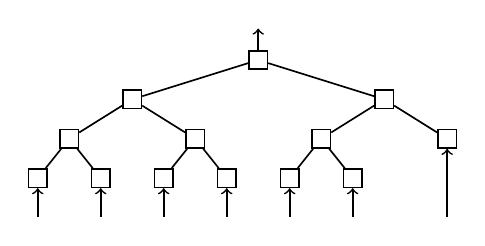
\begin{tikzpicture}
    [level distance=5mm, 
    level 1/.style={sibling distance=32mm},
    level 2/.style={sibling distance=16mm},
    level 3/.style={sibling distance=8mm},
    level 4/.style={sibling distance=4mm},
    semithick,
    every node/.style={draw=black}]
    \node[semithick] (root) {}
    child {node{} 
      child {node{}
        child {node{}}
        child {node{}}
      }
      child {node{}
        child {node{}}
        child {node{}}
      }
    }
    child {node{} 
      child {node{}
        child {node{}} 
        child {node{}}
      }
      child {node{}}
    };
    \draw[<-] (root-1-1-1) -- +(0,-.5);
    \draw[<-] (root-1-1-2) -- +(0,-.5);
    \draw[<-] (root-1-2-1) -- +(0,-.5);
    \draw[<-] (root-1-2-2) -- +(0,-.5);
    \draw[<-] (root-2-1-1) -- +(0,-.5);
    \draw[<-] (root-2-1-2) -- +(0,-.5);
    \draw[<-] (root-2-2)   -- +(0,-1);
    \draw[->] (root) -- + (0,.4);
  \end{tikzpicture}
  }
  \caption{Simulating an $n$-input AND-gate by several 2-input AND-gates}
  \label{fig:complete-binary-tree}
\end{figure}

The bottom level consists of at most $\frac{n}{2}$ AND-gates. The second-to-bottom level consists of at most $\frac{n}{4}$ gates. The next level has at most $\frac{n}{8}$ gates, and so forth. Thus, the total number of gates used is at most $\sum_{i=1}^{\log n} \frac{n}{2^i}\leq n$.

Thus, for one AND-gate that has $n$ inputs, we can construct a sub-circuit consisting of at most $n$ gates such that this sub-circuit resembles the computation of the original AND-gate. The size increased by a polynomial factor (in the number of inputs of the original gate). 

For other types of gates, we can use similar constructions.

Since any gate can have at most as many inputs as there are gates in the whole circuit, the size of the total circuit increases by a polynomial factor in the size of the circuit.

Note that this idea does not only work for AND gates, but also for other gates. In particular, it is working for splitter gates (as introduced in section \ref{sec:introducing-splitters}).

\subsection{How a dealer is ``bound'' to a commited value}
\label{sec:dealer-bound-to-commited-value}

In section \ref{sec:building-blocks-for-the-protocol} we said that the dealer is bound to his shared value once he commited to it. Of course, there are several ways to implement this, but we will briefly describe one from \cite{lecture-notes-goldwasser-bellare}.

Therefore, we use some one-way collision-free hash function $H$ (a one-way function is a function that can be easily evaluated, but whose inverse is very complicated or impossible to compute). Then, if we want to commit to some value $x$, we can send as a ``promise'' the value $y=H(x)$. Note that -- informally spoken -- nobody is able (at least not in feasible time) to find another value $x\neq y$ with $H(x)=H(x')=y$.

This way, we are bound to the value $x$ since we published $y=H(x)$ already, but can not find another value that yields $y$ when we apply $H$ to it. Thus, if we later publish our secret $x$, the other players just need to check whether they obtain $y$ when they apply $H$ to it. This way, we can not change our mind without being caught.

\subsection{The basic idea of secret sharing}
\label{sec:appendix-basic-idea-secret-sharing}

Consider the following basic idea for secret sharing. Assume you have some bit $s$ that you want to share among three players such that no player con reconstruct the value on her own (but they should be able to reconstruct it alltogether). 

Then, you could toss two coins yielding random bits $s_1$ and $s_2$. Moreover, you construct a third bit $s_3=s_1\oplus s_2\oplus s$. Note that then $s=s_1\oplus s_2 \oplus s_3$. Then you give $s_1$ to player 1, $s_2$ to player 2 and so forth. Afterwards the three players can -- collaboratively -- reconstruct the value $s$, but none of them can do so on her own.

This is -- of course -- a very simple scheme, that only works if all players are honest and if \emph{all} players join the collaborative computation.

However, there are more sophisticated techniques (e.g. relying on polynomials over finite fieds like $\mathbb Z_p$ for some prime $p$) that allow a certain amount of dishonest players and still work. 

For more information on that topic, please refer to \cite{shamir_secret_sharing}.

\subsection{Collaboraive coin flipping -- basic idea}
\label{sec:appendix-coin-flipping}

Taking the XOR (evaluating securely and secretly) of all these bits returns the random bit generated by all the participants in common. This computation (XOR on any number of bits) can be done in a constant number of rounds and using only polynomial amount of communication. This can be seen e.g. by a deeper investigation of the arguments in \cite{beaver-verifiable-secret-sharing} (according to \cite{Beaver1990}).

From now on, we use the symbol $\oplus$ to denote the XOR-computation. Even if XOR is usually defined on single bits only, we apply this function to bit strings bit-wise (e.g. $1100\oplus1001=0101$).

\subsection{Why the use of pseudorandom generators?}
\label{sec:appendix-why-pseudorandom-generators}

Let us for a moment consider equation (\ref{eq:gate-label-definition-with-output}) and propose the following question: The output of $G_0$ resp. $G_1$ on some $k$-bit string is a binary string of length $nk+1$. So, one might argue that it would be simpler to work directly on the signals $\sigma=\sigma_1\dots\sigma_n a$ and $\tau=\tau_1\dots\tau_n b$ instead of first splitting up the signals into its components and then considering $G_b(\sigma_i)$ and $G_a(\tau_j)$, respectively.

While this simplification would be useful if we were just interested in correctness, but when this is done, we loose privacy. That is, a player possibly can deduce the semantics of some signals -- which is something we strictly wanted to prevent.

To see this, consider a simple AND-gate (input wires $\alpha$ and $\beta$, output wire $\gamma$). Assume we know the left incoming signal $\sigma^\alpha$ to represent semantics $\mathbf{0}$ and has parity $a$ (similar, $\sigma^\beta$ has parity $b$). Then, we can surely say that the outgoing signal $\sigma^\gamma$ is also $\mathbf{0}$. If we would directly operate on the signals (i.e. without random generators), we could -- since we know all table entries for the gate -- deduce the signal for $\beta$ with parity $1-b$ (by simply considering the table entry $A^g_{a(1-b)}$). That is, we then would know all signals for wire $\beta$.

Then we do the same the other way around and compute all signals for wire $\alpha$. This enables us to ``test'' the gate with all combinations of odd and even signals. Since we knew that $\sigma^\alpha$ had parity $a$ and semantics $\mathbf{0}$, we could without problems try the other signal for $\alpha$ and see if the value of the wire $\gamma$ changes. This would enable us to deduce the semantics for the input wire $\beta$.

On the other hand, if we use pseudorandom generators, we can not deduce all the other signals, since the values $A^g_{ab}$ are scrambled. This prevents us from simply reconstructing the signals (and, thus, the semantics).

%------------------------------------------------------------------------------

%\nocite{*} %%% for now, print *all* references
\bibliographystyle{splncs}
\bibliography{literature.bib}

%\printbibliography{} %% bibLaTeX -- seemingly no good support in AucTeX
\end{document}

\message{ !name(seminar.tex) !offset(-1064) }
